\section{Deployment Considerations}
\label{sec:analysis_deployment}

A service can be designed from the ground up with security in mind, implementing the strongest encryption \& access control mechanisms possible, but if deployed incorrectly the functioning security of the service can be completely undermined. With that in mind, the \acrfull{dcs} represented a complex deployment scenario for a resource server.
\vskip 0.5em
The University of Glasgow does already provide Microsoft's SharePoint \citep{UofG2019} \& OneDrive \citep{UofG2019a} services as resource-sharing solutions to staff and students, however neither service offers truly granular access control \citep{Microsoft2019} and nor does either service offer a per-department service that the \acrshort{dcs} can implement for only its users. The \acrshort{dcs} is also large and complicated in structure, with over 500 users including both staff \& students with various roles, teams and groups (see \Cref{appendix:roles_users} for summary of \acrshort{dcs} structure).

This lack of granular access means that a user can not share a resource to all users enrolled in the same course, without manually inviting each user individually \textemdash\ a task that the user may not even have the information required to complete. By comparison, the \theResServer system would simply require creating a policy that grants access to users if and only if they have the attribute associated to that course, such as \textit{`enrolled\_course \= 2003'}.

The \theResServer system would have to cater to the needs of all users in the \acrshort{dcs} and be accessible for all users with relative ease. The two major components to be considered for deployment were the \acrfull{prs}, tasked with the digital storing, documenting \& distributing of all encrypted resources and the \acrfull{mks}, tasked with provisioning the system's master public \& private keys and later creating private keys for all users.

\subsection{Security of Public Resource Server}
\label{subsec:analysis_deployment_prs}

The \acrfull{prs} would need to be accessible to all users in the \acrshort{dcs} and able to process the uploading \& downloading of all encrypted resources. By design, the resource server would not be aware of the contents of any resources uploaded and would also be unable to execute any encryption or decryption tasks itself. The system would also reject uploads of any resources that are not encrypted, ensuring it is never aware of information contained in uploaded resources \textemdash\ hopefully helping to avoid the server becoming a target for attacks.

Physical deployment of the \acrshort{prs} should be simple, as the server must be publicly accessible to all users in the \acrshort{dcs} and requires a limited level of security. The server does not necessarily require access to the \acrfull{mks} (see \Cref{subsec:analysis_deployment_mks} and \Cref{fig:deployment_diagram}) and can instead rely on manual updates completed via physical transfer by \acrshort{dcs} Admin staff.
\vskip 0.5em
Depending on the desired use, the resource server may be deployed for internal-use only and kept within the \acrshort{dcs} network or for public access could be deployed with external access via the university's Campus network. Either scenario can be considered safe as the resources on the server are implicitly secure due to the employed at-rest \acrshort{abe}.

Regardless, once deployed the system should implement the university's SSO authentication system for basic access, which would help defend against denial-of-service attacks and other malicious attempts to disable or damage the system. Further consideration would need to be given to determining a suitable and effective method of completing backups of the encrypted resources but addressing that issue is outwith the scope of the project.

\subsection{Security of Master Key Server}
\label{subsec:analysis_deployment_mks}

Comparatively, the \acrfull{mks} represents the greatest risk to the \theResServer system, as the master \textbf{private} key stored within is capable of generating \& signing any private key desired. If the \acrshort{mks} becomes compromised, so does the entire system, since the master private key can then be maliciously used to generate any arbitrary decryption key as desired \textemdash\ eventually providing access to every encrypted resource.

To combat this risk, the \acrshort{mks} is designed to be kept `offline' after initial setup is complete and the whole system has been successfully provisioned. This drastically reduces attack vectors to the server and eliminates the risk of an external party gaining unauthorised digital access to the underlying system.

\begin{figure}[htp]
    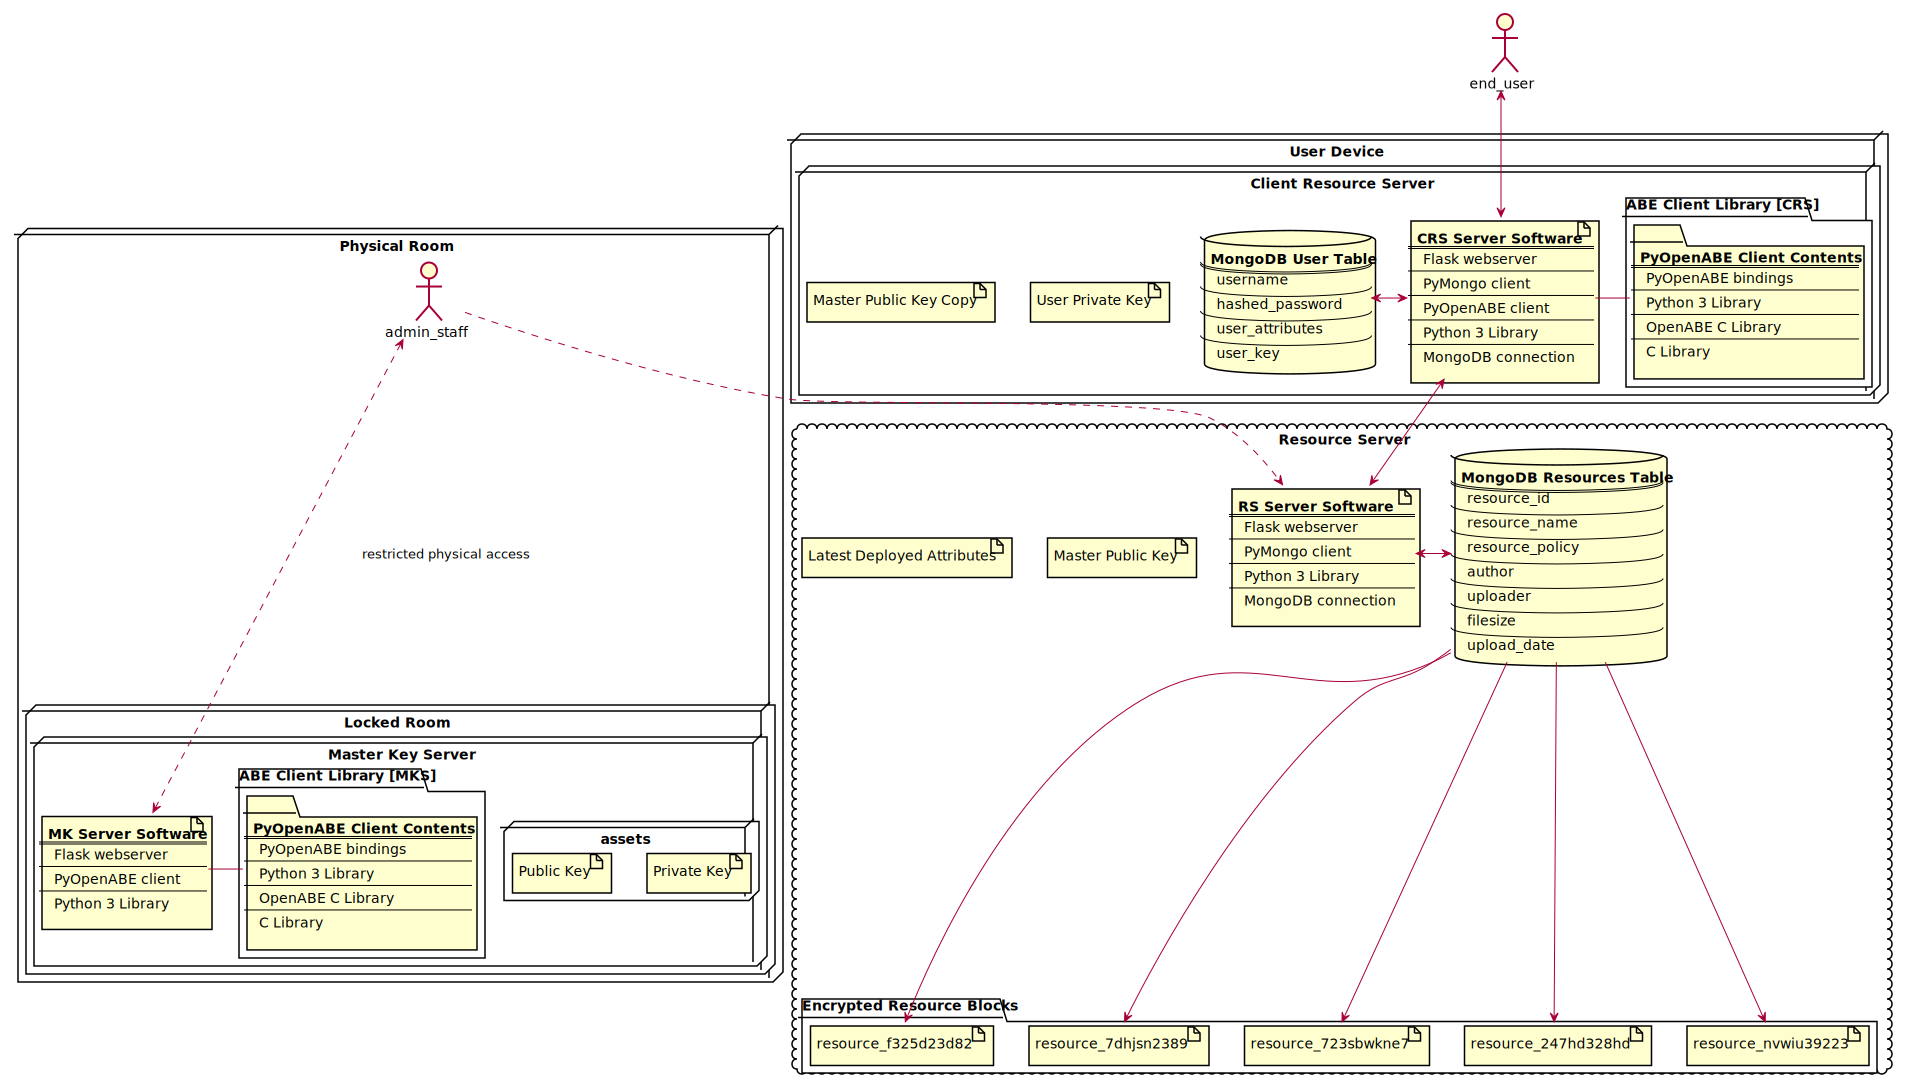
\includegraphics[width=\linewidth,keepaspectratio]{images/infrastructure/deployment.pdf}

    \caption{A deployment diagram of the \acrshort{dcs} \theResServer system. Both servers can be seen in context, with the \acrfull{mks} in its `offline' state and with physical access restricted to Admin staff. The \acrfull{prs} is also shown receiving physical updates from the \acrshort{mks} (handled by Admin Staff) and communicating with client software running on a user's local device.}

    \label{fig:deployment_diagram}
\end{figure}

Unfortunately, this still leaves physical access to the \acrshort{mks} as a concern, since the server will create any arbitrary user key it is instructed to. It was thus determined that physical access to the server must also be restricted, meaning the \acrshort{mks} would be deployed in a physically locked room with access only granted to \acrshort{dcs} Admin staff, as shown in \Cref{fig:deployment_diagram}.

Furthermore, the server would be built on a UNIX \acrshort{os} allowing for user authentication and system logging of events. This would ensure that even in the event of a physical breach of security, a rogue party could not access the \acrshort{mks} to issue new keys and that a rogue member of staff could not misuse the server to generate false keys without leaving an auditable trail.

\subsection{Issuing User Keys}
\label{subsec:analysis_deployment_iuk}

From \Cref{subsec:analysis_deployment_mks}, the \acrfull{mks} generates \& signs decryption keys for the \theResServer system, using the stored master \textbf{private} key. Further, as discussed in \Cref{subsec:analysis_abe}, the decryption keys for the system are private user keys which contain embedded attributes that describe a user in terms that are defined by the organisation, which in this case is the \acrshort{dcs}.

\begin{figure}[htp]
    \centering
    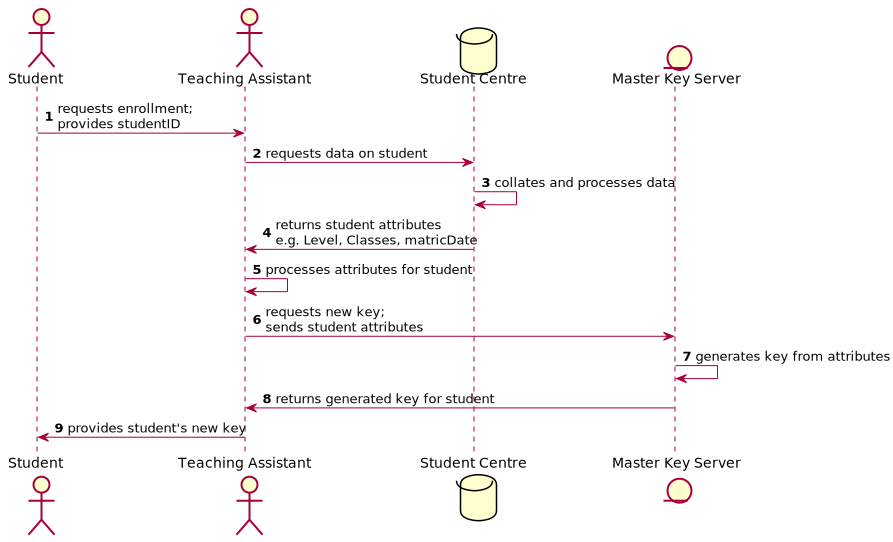
\includegraphics[width=\linewidth,keepaspectratio]{images/flow_of_info/enrollment_stu_sequence.pdf}

    \caption{A sequence diagram demonstrating the \theResServer enrolment process for a student.}

    \label{fig:enrolment_diagram}
\end{figure}

For a user to start using the \theResServer system, they must enrol in the system by having a member of the \acrshort{dcs} Admin staff generate \& sign a new user key with their personal details from the \acrshort{mks}, see \Cref{fig:enrolment_diagram} and Appendix \ref{appendix:enrolment_diagram}.

Where the student can be seen requesting a user key \#1 (and providing their student ID) from the \acrshort{dcs} Teaching Assistant, whom verifies the student's identity and then retrieves their details \#2 from the Student Centre (or MyCampus) system. The Teaching Assistant then processes the returned attributes \#5 for the Master Key Server, and then requests a new key \#6 by providing the student's attributes. The Master Key Server can be seen processing \#7 and then returning the newly generated key \#8 to the Teaching Assistant, whom finally provides the key to the student.

The key is created with attributes that should be retrieved from a department system such as MyCampus for students or the HR/Payroll system for staff. The \acrshort{mks} would be designed to \textit{validate} the attributes of a new user to ensure compatibility with encrypted resources and that all generated user keys are comparable.
\vskip 0.5em
However, the \acrshort{mks} would not be designed to \textit{verify} the attributes of a new user, since it is assumed that the Admin staff are responsible for verifying both the identity of a user and that the attributes about to be assigned to them are correct. The server would thus, implicitly trust that any inputs it receives have been verified and therefore, once validated would produce a new key; meaning both physical and login access to the server \textit{must only} be granted to trained members of staff.

In order for a new user key to be provided to the relevant user, the Admin staff member must physically transfer the newly created key from the master server key to the user via some form of hardware storage such as a provided USB flash drive. Care would have to be taken to ensure that the \acrshort{mks} does not become infected from malicious storage devices that might be provided by an unaware user or 3rd party.
